% --------------------------------------------------------------
\begin{frame}[fragile]
  \frametitle{Previous Work}
  \begin{itemize}
    \item Oak Ridge AHTR - unnecessary (Varma, Holcomb, et al.)
    \item COMSOL TH response analysis (Huff, Scarlat)
    \item Algebraic, 1-group LOFC neutronics analysis (Cisneros)
    \item Algebraic, 1-group RIA neutronics analysis (Greenspan, Fratoni)
  \end{itemize}

\end{frame}

% --------------------------------------------------------------
\begin{frame}[fragile]
  \frametitle{Unnecessary?}
  \begin{itemize}
    \item characterization of coolant, metal structure response
    \item characterization of startup strategy
    \item analysis of reactivity insertion behavior
    \item NRC required
  \end{itemize}
\end{frame}

% --------------------------------------------------------------
\begin{frame}[fragile]
  \frametitle{PB-FHR LOFC}
  Based on linear approximation, two coefficients, linear dT approximations.?
\end{frame}

% --------------------------------------------------------------
\begin{frame}[fragile]
  \frametitle{PB-FHR RIA}
  \$2 of reactivity insertion, max fuel temperature ~1200C. This is low enough for fuel survival.

  Based on linear approximation, two coefficients, linear dT approximations.?
\end{frame}

% --------------------------------------------------------------
\begin{frame}[fragile]
  \frametitle{Design Point?}

  \begin{figure}[htbp!]
    \begin{center}
      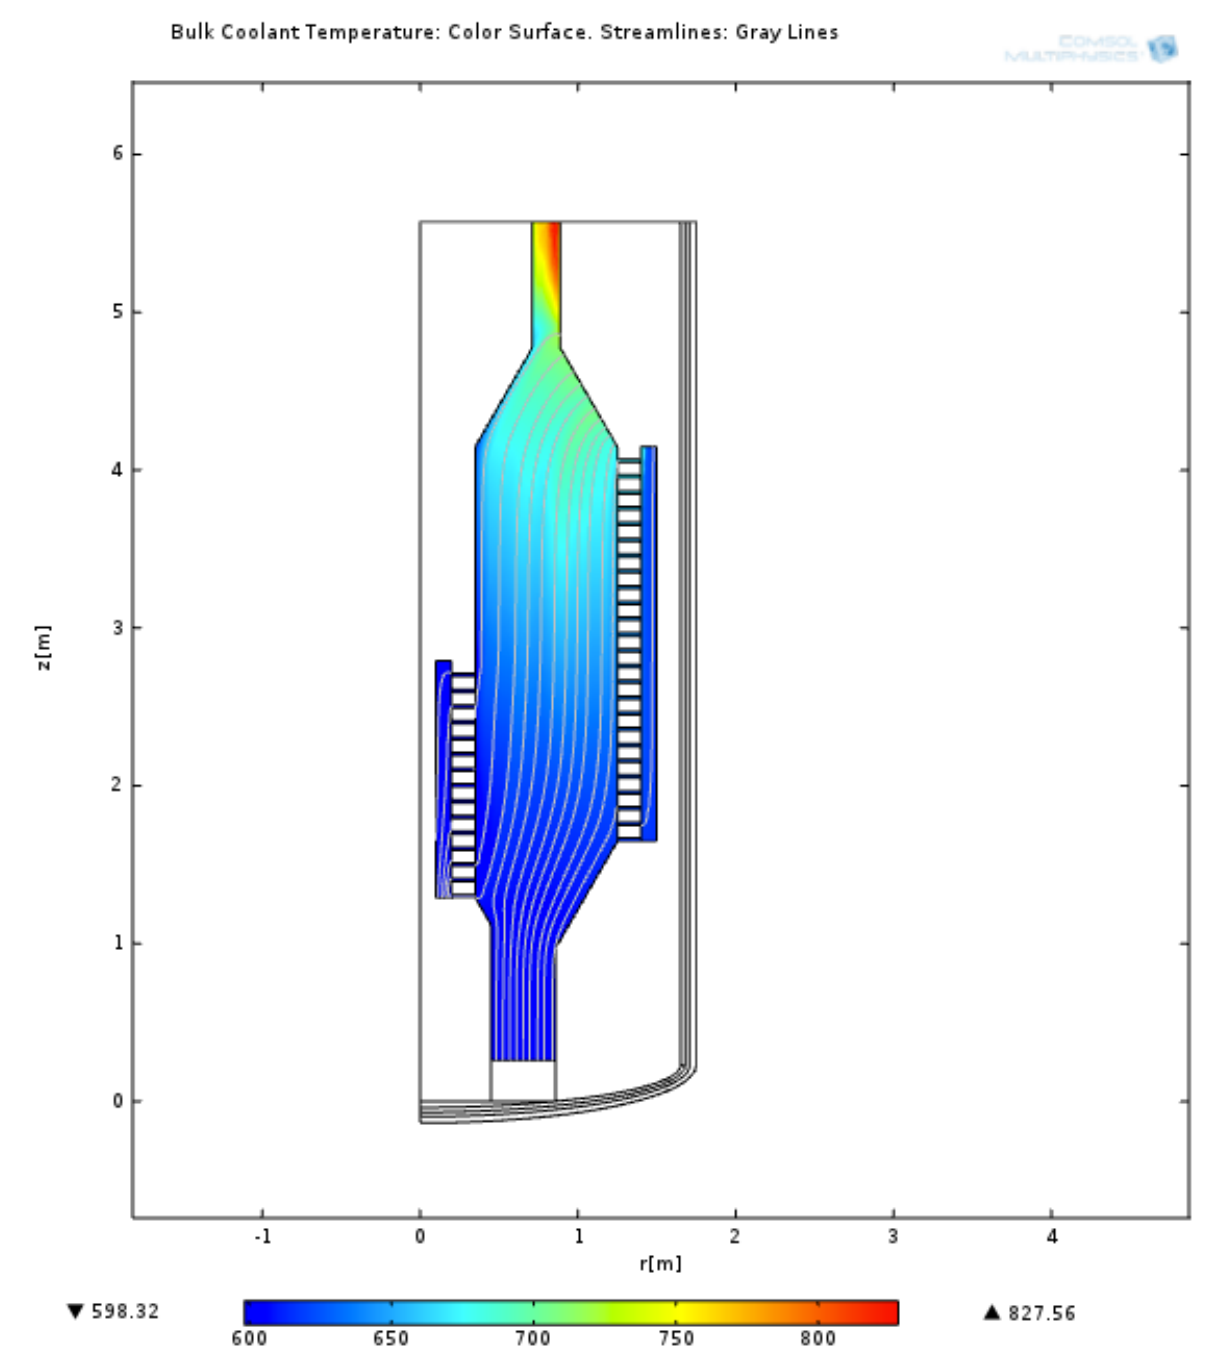
\includegraphics[height=0.8\textheight]{./priorart/coolant_temps_200_deg_rise.eps}
    \end{center}
    \caption{For 200 degree temperature rise design point across the core.}
    \label{fig:200degrise}
  \end{figure}
\end{frame}

